\subsection{Recap: Conways Law}
\begin{frame}{\insertsubsection}
	\begin{fancycolumns}[animation=none]
		\nextcolumn
		\vspace{-8mm}
		\href{https://twitter.com/conways_law}{\pic[width=\linewidth,trim=0 50 0 0,clip]{people/melvin-conway}}
		\vspace{-7mm}
		
		\begin{note}{Melvin E. Conway (1968) \mysource{\href{http://www.melconway.com/Home/Committees_Paper.html}{melconway.com}}}
			\mycite{Any organization that designs a system [...] will produce a design whose structure is a copy of the organization's communication structure.}
		\end{note}
	\end{fancycolumns}
\end{frame}

\subsection{Federated Software Architecture}
\begin{frame}{\insertsubsection\ \mytitlesource{\staron}}
	\begin{fancycolumns}[columns=3,widths={5,90,5},animation=none]
		\nextcolumn
		\myexampletight{}{\centering\staronlink{\pic[width=\linewidth,page=75,trim=60 430 60 60,clip]{automotive/S21}}}
		\nextcolumn
	\end{fancycolumns}
\end{frame}

\begin{frame}{\insertsubsection\ \mytitlesource{\vdovic}}
	\mydefinitiontight{Bus Systems for Automotive Systems}{\vdoviclink{\pic[width=\linewidth,page=3,trim=40 530 40 85,clip]{automotive/VBP-Access19}}}
\end{frame}

\xkcdframe{2212}

\subsection{Centralized Software Architecture}
\begin{frame}{\insertsubsection\ \mytitlesource{\staron}}
	\begin{fancycolumns}[columns=3,widths={5,90,5},animation=none]
		\nextcolumn
		\myexampletight{}{\centering\staronlink{\pic[width=\linewidth,page=78,trim=50 480 50 60,clip]{automotive/S21}}}
		\uncover<2->{\mynote{}{redundancy still needed for the fail safe mode}}
		\nextcolumn
	\end{fancycolumns}
\end{frame}

\begin{frame}{\insertsubsection\ \mytitlesource{\vdovic}}
	\myexampletight{Bus Systems in Use}{
		\vdoviclink{\pic[width=\linewidth,page=8,trim=40 670 40 85,clip]{automotive/VBP-Access19}}
		\vdoviclink{\pic[width=\linewidth,page=8,trim=40 402 40 217,clip]{automotive/VBP-Access19}}
	}
\end{frame}

\subsection{AUTOSAR: Standardization of Software Architectures}
\begin{frame}{\insertsubsection\ \mytitlesource{\staron}}
	\begin{fancycolumns}
		\begin{note}{Motivation}
			\begin{itemize}
				\item more efficient collaboration between different OEMs and tiers \deutsch{Automobilhersteller und Zulieferer}
				\item easier exchange of hardware
				\item common components
				\item common operating system
			\end{itemize}
		\end{note}
		\nextcolumn
		\begin{definition}{AUTOSAR}
			\begin{itemize}
				\item \emph{ATU}omotive \emph{O}pen \emph{S}ystem \emph{AR}chitecture
				\item reference architecture + development methodology + AUTOSAR platform
				\item \emph{AUTOSAR Classic Platform}\\ for traditional mechatronic systems (e.g., doors, air conditioning)
				\item \emph{AUTOSAR Adaptive Platform}\\ for modern system (e.g., autonomous driving, connectivity)
			\end{itemize}
		\end{definition}
	\end{fancycolumns}
\end{frame}

\subsection{Example Architecture of a Modern Car}
\begin{frame}[b]{\insertsubsection\ \mytitlesource{\vdovic}}
	\begin{fancycolumns}[columns=3,widths={5,80,5},animation=none]
		\nextcolumn
		\vdoviclink{\pic[width=\linewidth,page=7,trim=55 395 60 75,clip]{automotive/VBP-Access19}}
		\nextcolumn
	\end{fancycolumns}
\end{frame}

%\subsection{Forschung zu Automotive Software Engineering}
%\begin{frame}{\insertsubsection\ \mytitlesource{\asesurvey}}
%	\begin{fancycolumns}[widths={60}]
	%		\asesurveylink{\includegraphics[width=\linewidth,page=12,trim=35 410 35 60,clip]{HBP+-JSS17}}
	%	\nextcolumn
	%		\asesurveylink{\includegraphics[width=\linewidth,page=12,trim=320 165 35 420,clip]{HBP+-JSS17}}
	%	\end{fancycolumns}
%\end{frame}

\subsection{Recap: Architectural Patterns}
\begin{frame}{\insertsubsection\ \deutsch{Architekturmuster}}
	\slideArchitecturalPattern
\end{frame}

\subsection{Layered Architecture}
\begin{frame}{\insertsubsection\ \mytitlesource{\staron}}
	\begin{fancycolumns}[animation=none]
		\nextcolumn
		\vspace{-10mm}
		\myexampletight{Reference Architecture for Autonomous Driving}{\centering\staronlink{\pic[width=.9\linewidth,page=55,trim=75 250 75 60,clip]{automotive/S21}}}
	\end{fancycolumns}
\end{frame}

\subsection{Pipe-and-Filter Architecture}
\begin{frame}{\insertsubsection\ \mytitlesource{\staron}}
	\begin{fancycolumns}[columns=3,widths={5,90,5},animation=none]
		\nextcolumn
		\myexampletight{Image Processing}{\centering\staronlink{\pic[width=\linewidth,page=59,trim=65 250 65 285,clip]{automotive/S21}}}
		\nextcolumn
	\end{fancycolumns}
\end{frame}

\subsection{Client-Server Architecture}
\begin{frame}{\insertsubsection\ \mytitlesource{\staron}}
	\begin{fancycolumns}[columns=3,widths={5,66,5},animation=none]
		\nextcolumn
		\myexampletight{Fleet Management \deutsch{Flottenmanagement}}{\centering\staronlink{\pic[width=\linewidth,page=60,trim=75 265 85 245,clip]{automotive/S21}}}
		\mynote{}{Telematics = Telecommunication + Informatics}
		\nextcolumn
	\end{fancycolumns}
\end{frame}

\subsection{Publisher-Subscriber Architecture}
\begin{frame}{\insertsubsection\ \mytitlesource{\staron}}
	\begin{fancycolumns}[columns=3,widths={5,75,5},animation=none]
		\nextcolumn
		\myexampletight{Speed Control}{\centering\staronlink{\pic[width=\linewidth,page=61,trim=65 285 75 250,clip]{automotive/S21}}}
		\mynote{Publisher-Subscriber Architecture}{similar to observer pattern but on architectural level}
		\nextcolumn
	\end{fancycolumns}
\end{frame}

\begin{frame}[b]{Recap: Gordon Bell}
	\begin{fancycolumns}[animation=none]
		\nextcolumn
		\vspace{-15mm}
		\href{https://en.wikipedia.org/wiki/File:Gordon_Bell.jpg}{\pic[width=\linewidth,trim=175 0 0 0,clip]{people/gordon-bell}}
		\vspace{-7mm}
		
		\begin{note}{Gordon Bell \mysource{\href{https://dl.acm.org/doi/10.1145/1968.381154}{Bentley 1984}}}
			\mycite{The cheapest, fastest, and most reliable components are those that aren’t there.}
		\end{note}
	\end{fancycolumns}
\end{frame}

